\documentclass[aspectratio=169]{beamer}


%%% Style
%%% Gabarit de présentation du DMS
\RequirePackage{graphicx}
\usepackage{colortbl}

\usepackage{tikz}

%%% Couleurs
\definecolor{bleu-udem}{RGB}{0, 107, 182}
\definecolor{gris-udem}{RGB}{102, 102, 102}
\definecolor{rouge}{RGB}{204, 0, 0}
\definecolor{vert}{RGB}{153, 204, 0}

\definecolor{intact-red}{RGB}{192, 0, 0}
\definecolor{intact-blue}{RGB}{24, 168, 166}

\usecolortheme{lily}  % désinstalle les couleurs par défaut
\setbeamercolor*{normal text}{fg=black,bg=white}
\setbeamercolor*{alerted text}{fg=rouge}
\setbeamercolor*{example text}{fg=vert}
\setbeamercolor*{structure}{fg=black}

\setbeamercolor*{block title}{fg=white,bg=gris-udem}
\setbeamercolor*{block title alerted}{fg=white,bg=gris-udem}
\setbeamercolor*{block title example}{fg=white,bg=gris-udem}

\setbeamercolor*{block body}{bg=black!10}
\setbeamercolor*{block body alerted}{bg=black!10}
\setbeamercolor*{block body example}{bg=black!10}

\setbeamercolor{item}{fg=bleu-udem}
\setbeamercolor{background canvas}{bg=gris-udem!5}


%%% Liens
\hypersetup{
  colorlinks=true,
  pdfnewwindow=true,
  linkcolor=gris-udem,
  citecolor=bleu-udem,
  filecolor=bleu-udem,
  urlcolor=bleu-udem
}


%%% Canva
\newlength{\textmarginL}
\newlength{\textmarginR}
\setlength{\textmarginL}{7.5mm}
\setlength{\textmarginR}{3.5mm}
%\setlength{\textmarginL}{0mm}
%\setlength{\textmarginR}{0mm}
\setbeamersize{text margin left=\textmarginL, text margin right=\textmarginR}
\newlength{\titleseparator}
\setlength{\titleseparator}{.71\paperwidth}  % distance entre le côté gauche et la barre horizontale (Page titre)
\newenvironment{changemargin}[2]{%
  \begin{list}{}{%
    \setlength{\topsep}{0pt}%
    \setlength{\leftmargin}{#1}%
    \setlength{\rightmargin}{#2}%
    \setlength{\listparindent}{\parindent}%
    \setlength{\itemindent}{\parindent}%
    \setlength{\parsep}{\parskip}%
  }%
  \item[]}{\end{list}}

%%% Images et logo
\newcommand{\insertslidelogo}{\rule{0pt}{.14\paperheight}} % .14\paperheight = .22\paperwidth
\newcommand{\slidelogo}{
  \renewcommand{\insertslidelogo}{
	
\includegraphics[height=.14\paperheight]{figures/template/titlepage_background}
  }
}
\newcommand{\inserttitlelogo}{\rule{0pt}{.16\paperheight}}  % .16\paperheight = .25\paperwidth
\newcommand{\titlelogo}{
  \renewcommand{\inserttitlelogo}{
	
\includegraphics[height=0.16\paperheight]{figures/template/titlepage_background}
  }
}
\newcommand{\inserttitleimage}{\rule{0pt}{.28\paperheight}}
\newcommand{\titleimage}[1]{
  \renewcommand{\inserttitleimage}{
  \includegraphics[height=.28\paperheight, keepaspectratio=true]{#1}
  }
}

%%% Page titre
\setbeamertemplate{title page}{

\begin{changemargin}{-\textmarginL}{-\textmarginR}
%\begin{tabular}{@{}r!{\color{bleu-udem}\vline}@{}l@{}}
% & \inserttitlelogo\\
%\inserttitleimage & \\
%\rule{0pt}{20pt}
%\parbox{\titleseparator}{\flushright\Large{\inserttitle}} & \\
%\parbox{\titleseparator}{\flushright\small{\insertsubtitle}}  & \\
%\rule{0pt}{24pt}
%\parbox{\titleseparator}{\flushright\insertauthor} & \\
%\parbox{\titleseparator}{\flushright\insertinstitute}  & \\
%\rule{0pt}{18pt}
%\parbox{\titleseparator}{\flushright\small{\insertdate}} & \\
%\end{tabular}
\vspace{-9pt}
\begin{tikzpicture}
	\draw (0, 0) node[inner sep=0] {
\includegraphics[width=\paperwidth, height=1.02\paperheight]{figures/template/titlepage_background}};
	\draw (0, 2) node {\parbox{\titleseparator}{\centering \color{white} \Huge{\inserttitle}}};
	\draw (-2, -0.5) node {\parbox{\titleseparator}{\centering \color{white} \Large{\insertauthor}}};
	\draw (-2, -1.25) node {\parbox{\titleseparator}{\centering \color{white} \insertinstitute}};
	\draw (-2, -2.) node {\parbox{\titleseparator}{\centering \color{white} \insertdate}};

\end{tikzpicture}
\end{changemargin}
}


%%% Entête
\setbeamertemplate{frametitle}{%
\vskip-33pt\parbox[c]{.68\paperwidth}{\large\insertframetitle}\vskip4pt%
}
\setbeamertemplate{headline}{%
\vspace{.14\paperheight}

\hspace{20pt}
\color{intact-blue}\rule{0.075\paperwidth}{0.5pt}
\hspace{-5pt}
\color{black}\rule{0.075\paperwidth}{0.5pt}
\hspace{-5pt}
\color{intact-red}\rule{.075\paperwidth}{.5pt}%
}


%%% Pied de page
\beamertemplatenavigationsymbolsempty
\newcommand{\numsubsectionname}{}
\newcommand{\showsubsection}{
  \renewcommand{\numsubsectionname}{%
	\thesection.\thesubsection \; \insertsubsection
  }
}
\newcommand{\insertfootlinetext}{}
\newcommand{\footlinetext}[1]{
  \renewcommand{\insertfootlinetext}{#1}
}
%\setbeamertemplate{footline}{
%{\hfill\color{bleu-udem}\rule{.98\paperwidth}{0.07pt}}%
%\vskip4pt%
%\color{gris-udem}%
%\rule{0.02\paperwidth}{0pt}%
%\numsubsectionname
%\hfill%
%\mbox{\insertfootlinetext\qquad\qquad\insertframenumber}%
%\rule{\textmarginR}{0pt}%
%\vskip4pt%
%}

\setbeamertemplate{footline}{

\hspace{12pt}
\begin{tikzpicture}
	\node[mark size=7.5pt,color=intact-blue] at (0,0) {\pgfuseplotmark{*}};
	\node[mark size=7.5pt,color=intact-red, opacity=0.9] at (0.25,0) {\pgfuseplotmark{*}};
	\draw (0.25, 0) node {\color{white} \insertframenumber};
\end{tikzpicture}
\vspace{12pt}
}




%%% Extensions utiles pour le français
\usepackage[french]{babel}
\usepackage[utf8]{inputenc}
\usepackage[T1]{fontenc}

\usepackage{xcolor}

%%% Extensions utiles pour les math
\usepackage{amsmath}
\usepackage{amsfonts}
\usepackage{bbold}
\usepackage{mathtools}

\DeclareMathOperator*{\argmin}{arg\,min}

%%% Extensions pour les figures
\usepackage{graphicx}
\usepackage{subfig}
\usepackage{tikz}

%%% for python scripts
\usepackage{listings}
\usepackage{verbatim}

%%% Bibliographie
\usepackage{bibentry}

%%% Informations sur la présentation
\author{Patrice B\'echard}
\institute[Intact]{
\small{Intact Data Lab} \\
\textit{patrice.bechard@intact.net}
}
\title{Pattern recognition avec des données géospatiales}
\date{19 janvier 2019}


%%% Préférences (Propre au thème du DMS)
\slidelogo
\titlelogo
%\titleimage{figures/deep_learning_v2.png}  % Image à afTficher sur la page titre
\footlinetext{  % À utiliser surtout pour les congrès
\insertshorttitle\quad\insertshortdate\quad\insertshortinstitute
}


\def\signed #1{{\leavevmode\unskip\nobreak\hfil\penalty50\hskip2em
  \hbox{}\nobreak\hfil(#1)%
  \parfillskip=0pt \finalhyphendemerits=0 \endgraf}}

\newsavebox\mybox
\newenvironment{aquote}[1]
  {\savebox\mybox{#1}\begin{quote}}
  {\signed{\usebox\mybox}\end{quote}}

\usepackage{ragged2e}


%%% Début
\begin{document}

% Title page

\begin{frame}[plain, t]
  \titlepage
\end{frame}

% Motivations

\begin{frame}{Motivation}
\centering
{\Large Pourquoi est-ce un problème intéressant?}
\vspace{.5cm}

\begin{itemize}
    \item Beaucoup de données GPS provenant des usagers
    \item On voudrait les utiliser pour
    \begin{itemize}
        \item Trouver des \textit{patterns} dans les habitudes de conduite des usagers
        \item Détecter des sections de routes dangereuses
        \item Optimiser le trajet le plus vide en fonction du traffic
        \item ...
    \end{itemize}
\end{itemize}
    
\end{frame}


\begin{frame}{Plan}
  \tableofcontents
\end{frame}

%%%%%%%%%%%%%%%%%%%%%%%%%%%%%%%%%%%%%%%%%%%%%%%%%%%%%%%%%%%%%%%%%%%%%%%%%%%%%%%%%%%%%%%%
% Open Street Map
%%%%%%%%%%%%%%%%%%%%%%%%%%%%%%%%%%%%%%%%%%%%%%%%%%%%%%%%%%%%%%%%%%%%%%%%%%%%%%%%%%%%%%%%

\section{Open Street Map}
\begin{frame}{Open Street Map (OSM) \cite{haklay2008openstreetmap}}

\begin{center}
{\LARGE Open Street Map}
\end{center}

\begin{columns}
\begin{column}{0.5\textwidth}
	
	\begin{itemize}
		\item Carte \textit{Open-Source} maintenue par les utilisateurs
		\item Contient des informations à propos des:
		\begin{itemize}
			\item segments de route
			\item intersections
			\item monuments
			\item ...
		\end{itemize}
		\item Contient un moteur de routage similaire à Google Maps 
		\item \url{https://www.openstreetmap.org/}
	\end{itemize}
\end{column}
\begin{column}{0.5\textwidth}  %%<--- here
    \begin{center}
     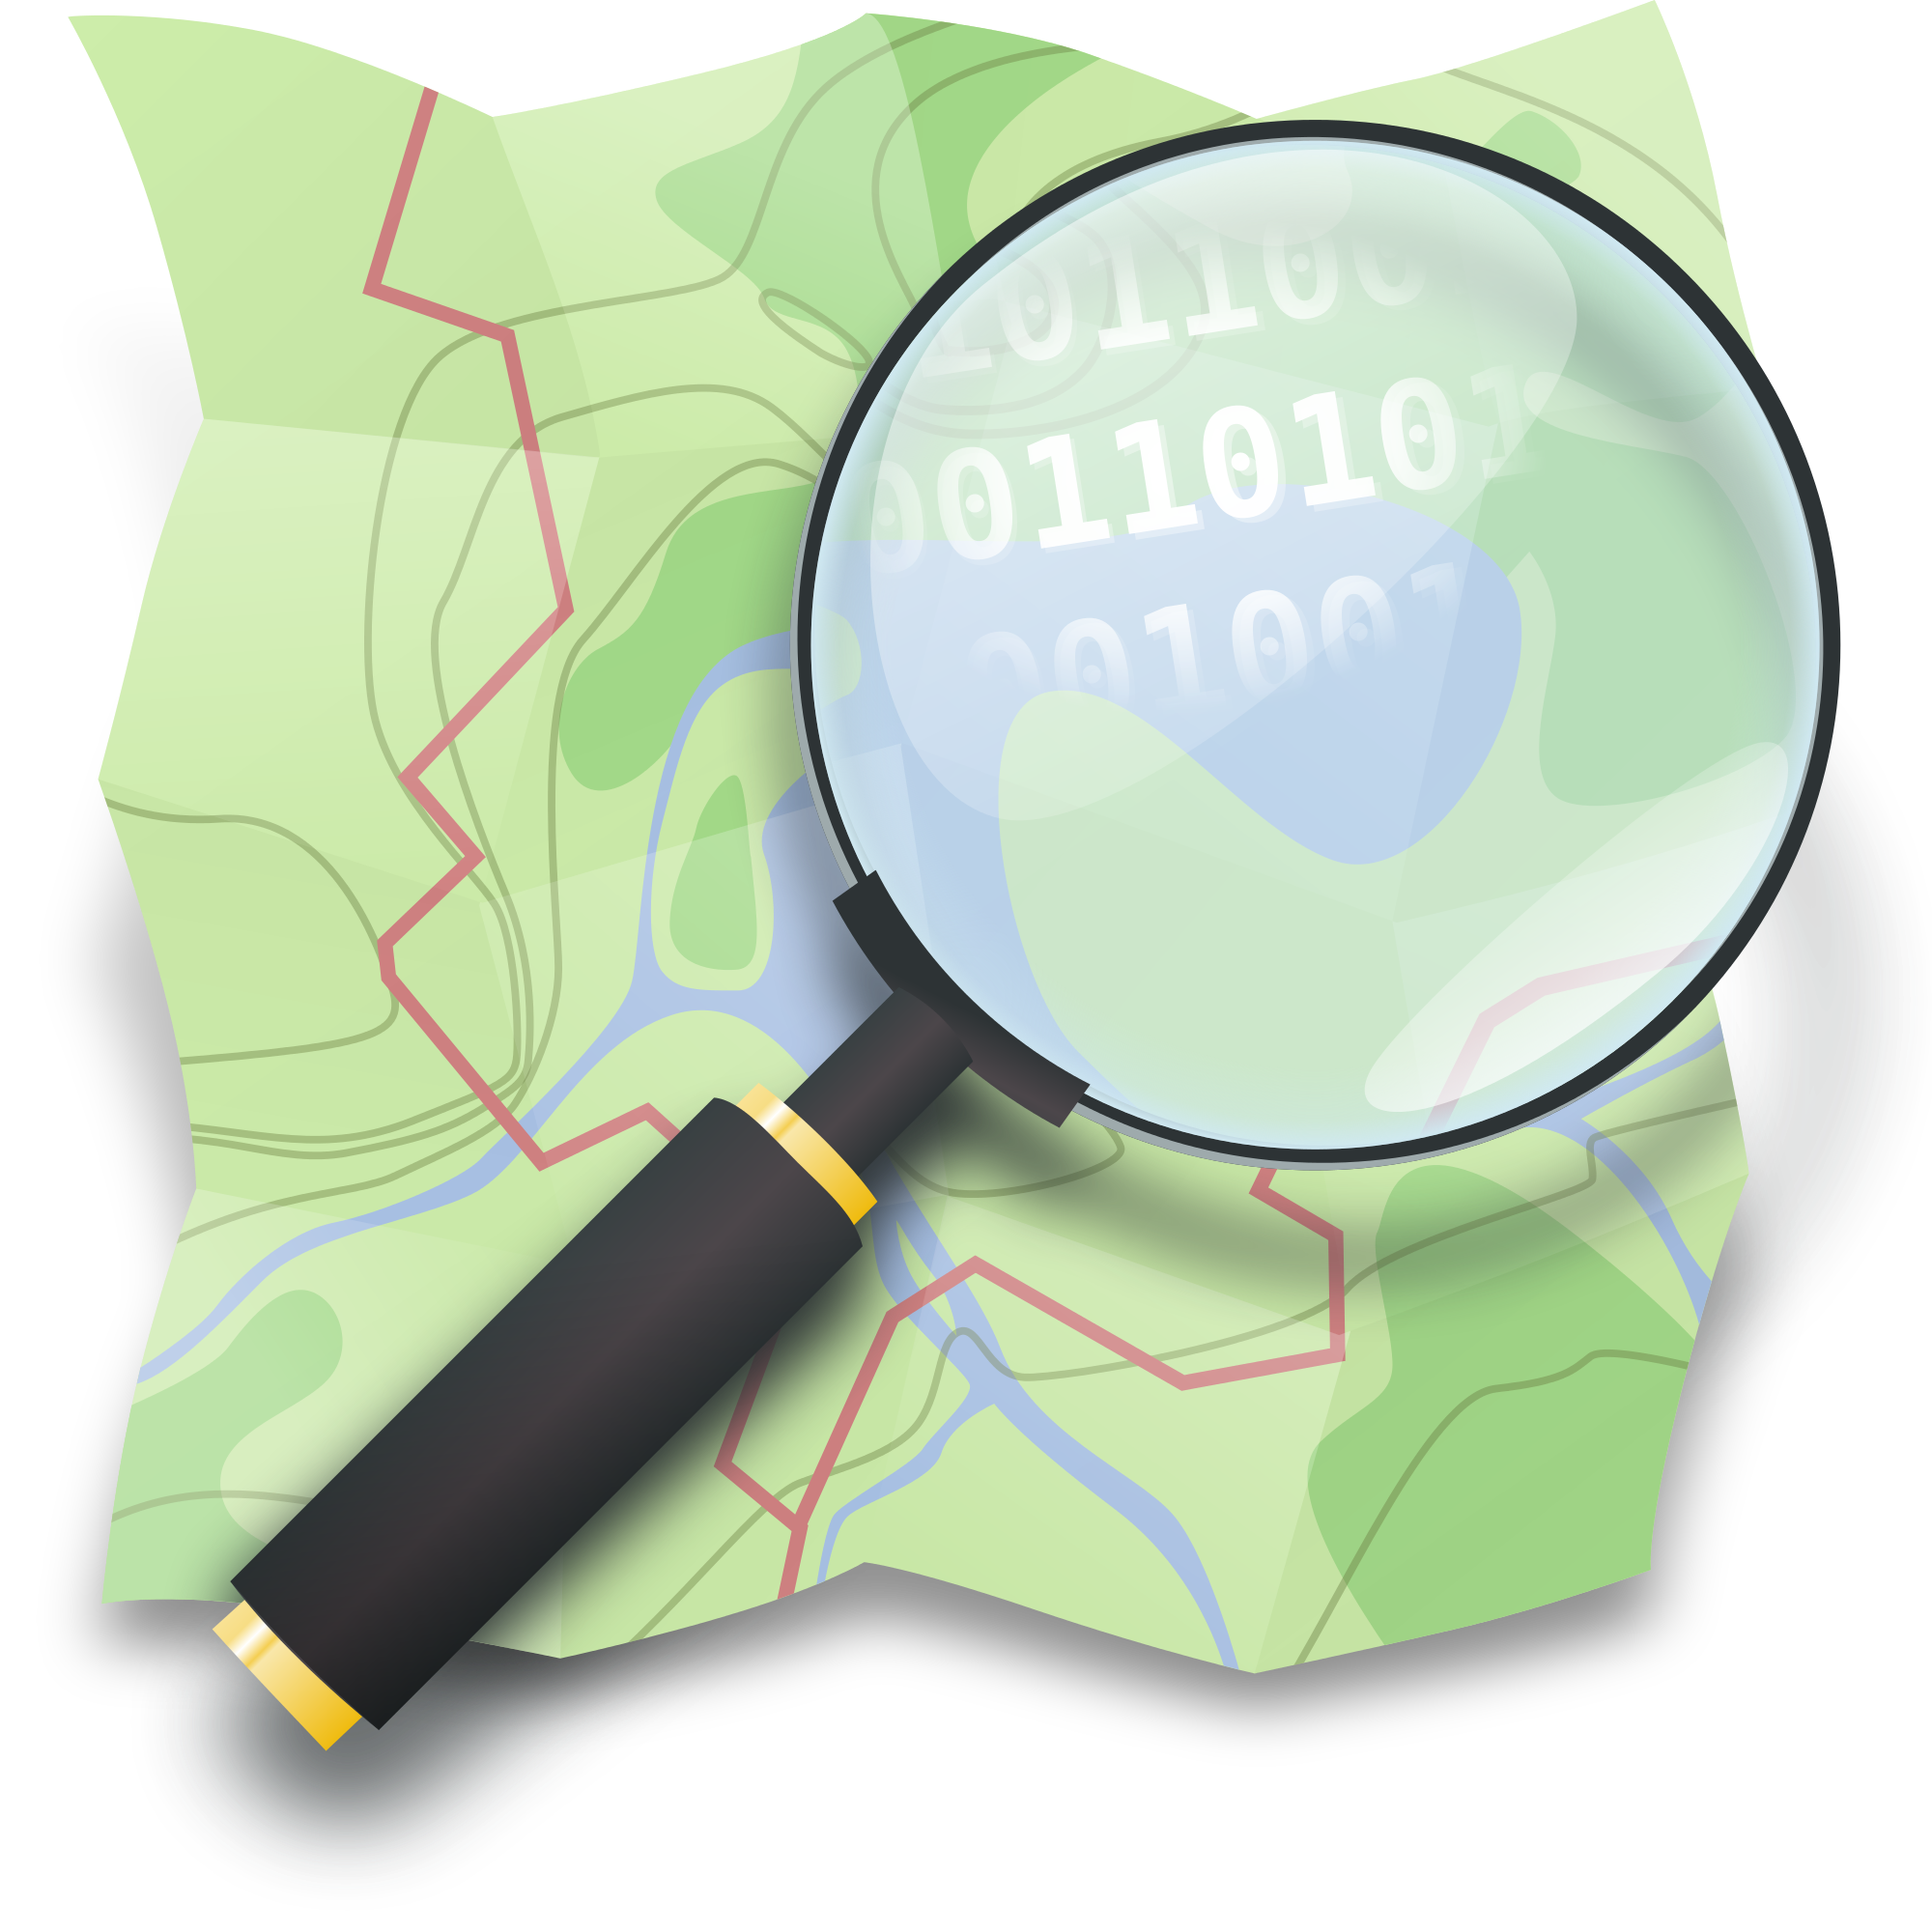
\includegraphics[width=0.7\textwidth]{figures/osm_logo.png}
     \end{center}
\end{column}
\end{columns}
\end{frame}

\begin{frame}{Open Street Map (OSM) \cite{haklay2008openstreetmap}}

{\Large Exemple : requête des objets à proximité}
\centering
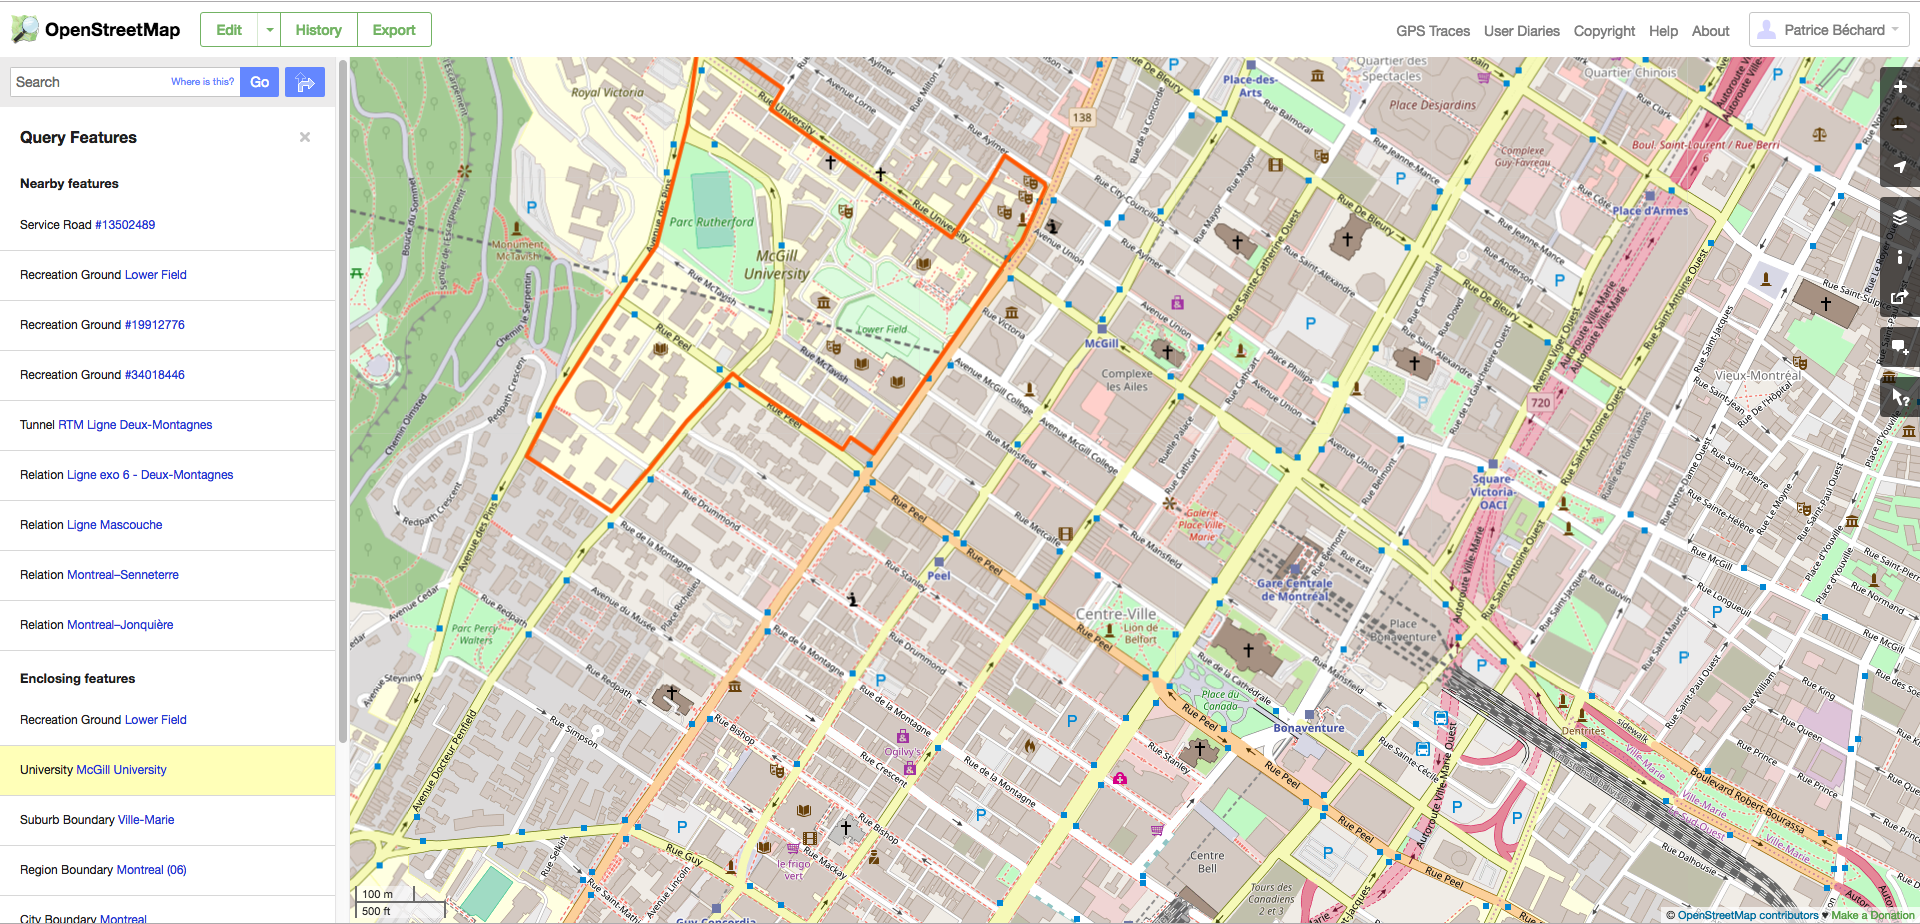
\includegraphics[width=0.85\textwidth]{figures/osm_query}

\end{frame}

\begin{frame}{Open Street Map (OSM) \cite{haklay2008openstreetmap}}

{\Large Exemple : Trouver le trajet optimal entre deux points}
\centering
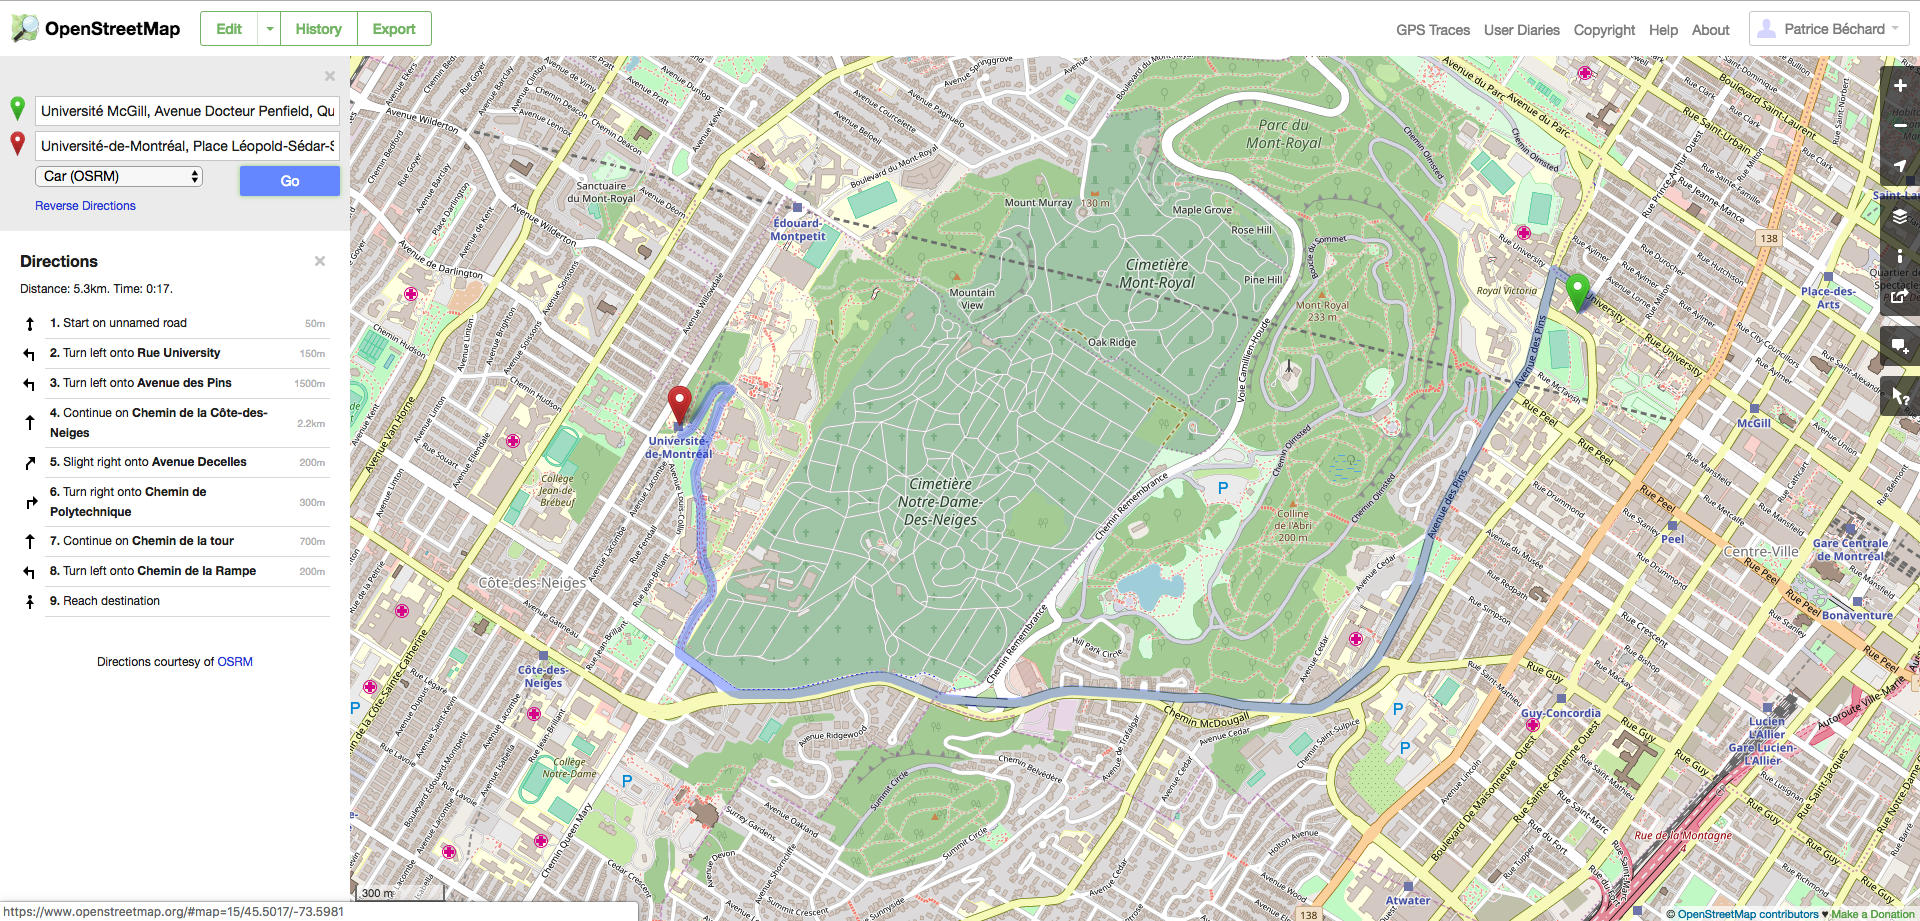
\includegraphics[width=0.85\textwidth]{figures/osm_routing}

\end{frame}

%%%%%%%%%%%%%%%%%%%%%%%%%%%%%%%%%%%%%%%%%%%%%%%%%%%%%%%%%%%%%%%%%%%%%%%%%%%%%%%%%%%%%%%%
% OSMnx
%%%%%%%%%%%%%%%%%%%%%%%%%%%%%%%%%%%%%%%%%%%%%%%%%%%%%%%%%%%%%%%%%%%%%%%%%%%%%%%%%%%%%%%%

\section{Construire et visualiser le réseau routier avec OSMnx}

\begin{frame}{OSMnx \cite{boeing2017osmnx}}

\begin{center}
{\LARGE OSMnx}
\end{center}

\begin{columns}
\begin{column}{0.75\textwidth}
	
	\begin{itemize}
		\item Librairie Python \textit{open-source}
		\item Représente le réseau routier comme un graphe orienté
		\item Nous permet de :
		\begin{itemize}
			\item Créer le réseau routier d'un endroit défini
			\item Visualiser le réseau facilement
			\item Simplifier le réseau routier en supprimant les noeuds n'étant pas des intersections
			\item Calculer des statistiques à propos du réseau routier construit
			\item Trouver le chemin le plus cours entre deux noeuds du réseau
			\item ...
		\end{itemize}
		\item \url{https://github.com/gboeing/osmnx}
	\end{itemize}
\end{column}
\begin{column}{0.25\textwidth}  %%<--- here
    \begin{center}
     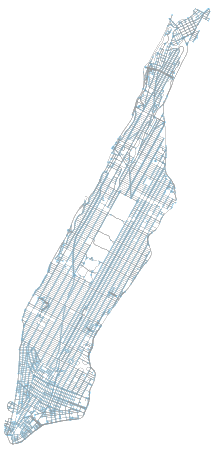
\includegraphics[width=0.8\textwidth]{figures/osmnx_manhattan}
     \end{center}
\end{column}
\end{columns}
\end{frame}

\begin{frame}{OSMnx \cite{boeing2017osmnx}}

{\Large Exemple : Créer le réseau routier de Verdun}
{\small \lstinputlisting[language=Python]{scripts/verdun_network.py}}
\centering

\includegraphics[height=4cm]{figures/verdun_network}

\end{frame}

\begin{frame}{OSMnx \cite{boeing2017osmnx}}

{\Large Exemple : Créer la forme de l'Île de Montréal}
{\small \lstinputlisting[language=Python]{scripts/montreal_shape.py}}
\centering
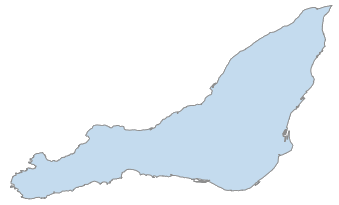
\includegraphics[height=4cm]{figures/montreal_shape}

\end{frame}

\begin{frame}{OSMnx \cite{boeing2017osmnx}}

{\Large Exemple : Créer un graphe à partir d'un \textit{bounding box}}
{\small \lstinputlisting[language=Python]{scripts/graph_from_bbox.py}}
\vspace{.5cm}
{\Large Exemple : Créer un graphe à partir d'un seul point GPS}
{\small \lstinputlisting[language=Python]{scripts/graph_from_point.py}}

\end{frame}

\begin{frame}{OSMnx \cite{boeing2017osmnx}}

{\Large Exemple : Calculer les statistiques d'un réseau routier}
{\small \lstinputlisting[language=Python]{scripts/osmnx_stats.py}}
{\small \verbatiminput{scripts/osmnx_stats_results.json}}

\end{frame}

\begin{frame}{OSMnx \cite{boeing2017osmnx}}

{\Large Exemple : Trouver le chemin le plus court entre deux endroits}
{\footnotesize \lstinputlisting[language=Python]{scripts/shortest_path.py}}

\end{frame}

\begin{frame}{OSMnx \cite{boeing2017osmnx}}

{\Large Exemple : Trouver le chemin le plus court entre deux endroits}
\centering
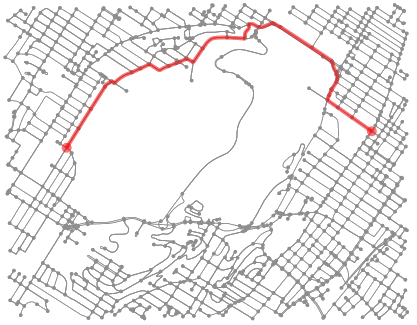
\includegraphics[width=0.5\textwidth]{figures/shortest_path}

\end{frame}

\begin{frame}{OSMnx \cite{boeing2017osmnx}}

{\Large Pour plus d'exemples et de fonctionnalités de OSMnx, consultez ces liens:}
\vspace{1cm}
\begin{itemize}
	\item \url{https://geoffboeing.com/2016/11/osmnx-python-street-networks/} (aperçu)
	\item \url{https://osmnx.readthedocs.io/en/stable/} (documentation)
	\item \url{https://github.com/gboeing/osmnx-examples/} (plus d'examples)
\end{itemize}

\end{frame}

%%%%%%%%%%%%%%%%%%%%%%%%%%%%%%%%%%%%%%%%%%%%%%%%%%%%%%%%%%%%%%%%%%%%%%%%%%%%%%%%%%%%%%%%
% GeoLife GPS Trajectories dataset
%%%%%%%%%%%%%%%%%%%%%%%%%%%%%%%%%%%%%%%%%%%%%%%%%%%%%%%%%%%%%%%%%%%%%%%%%%%%%%%%%%%%%%%%

\section{GeoLife GPS Trajectories Dataset}

\begin{frame}{GeoLife GPS Trajectories Dataset \cite{zheng2008understanding, zheng2010geolife, zheng2009mining}}

\begin{center}
{\LARGE GeoLife GPS Trajectories Dataset}
\end{center}

Ensemble de données contenant les trajectoires GPS de 191 usagers, la plupart aux alentours de Beijing, Chine.
\begin{itemize}
	\item \textbf{Nombre de trajets} : 18,670
	\item \textbf{Distance totale parcourue} : 1,292,951 km
	\item \textbf{Temps total} : 50,176 heures
\end{itemize}
\vspace{.5cm}
Pour un aperçu complet de l'ensemble de données :
\begin{itemize}
	\item \url{https://www.microsoft.com/en-us/research/wp-content/uploads/2016/02/User20Guide-1.2.pdf}
\end{itemize}

\end{frame}

%%%%%%%%%%%%%%%%%%%%%%%%%%%%%%%%%%%%%%%%%%%%%%%%%%%%%%%%%%%%%%%%%%%%%%%%%%%%%%%%%%%%%%%%
% Origin Clustering
%%%%%%%%%%%%%%%%%%%%%%%%%%%%%%%%%%%%%%%%%%%%%%%%%%%%%%%%%%%%%%%%%%%%%%%%%%%%%%%%%%%%%%%%

\section{Trouver les points d'intérêt à Beijing}

\begin{frame}{Trouver les points d'intérêt à Beijing}

\begin{center}
{\LARGE Trouver les points d'intérêt à Beijing}
\end{center}

On peut utiliser l'origine et la destination des trajet pour trouver les points d'intérêt à Beijing.

\begin{itemize}
	\item On utilise le GeoLife GPS Trajectories Dataset.
	\item On utilise les algorithmes de \textit{clustering} de la librairie python \textit{Scikit-Learn}\cite{pedregosa2011scikit}.
\end{itemize}
\end{frame}

\begin{frame}{Trouver les points d'intérêt à Beijing}

{\Large Qu'est-ce que le \textit{clustering}?}
\vspace{.5cm}

\begin{itemize}
	\item Type de problème d'apprentissage non-supervisé
	\item On essaie de trouver des groupes de données avec des propriétés similaires.
	\item Dans notre cas, on veut trouver les points GPS étant proche de chacun.
\end{itemize}
\vspace{.5cm}

On décide d'utiliser l'algorithme \textbf{DBSCAN}\cite{ester1996density} pour plusieurs raisons :
\begin{itemize}
	\item Les \textit{clusters} peuvent être de forme arbitraire
	\item Pas besoin de spécifier un nombre de \textit{clusters} manuellement
\end{itemize}
\end{frame}

\begin{frame}{Trouver les points d'intérêt à Beijing}

{\Large \textbf{Tâche} : trouver les 10 plus grands \textit{clusters} dans l'ensemble de données et les identifier}
\vspace{.5cm}
\\
{\Large \textbf{À faire}}:
\begin{enumerate}
	\item Regrouper les données avec l'algorithme DBSCAN
	\item Enlever les points ne faisant pas partie des 10 plus grands \textit{clusters}
	\item Trouver le centroïde de chaque \textit{cluster}
	\item Utiliser le géocodage inversé (reverse geocoding) pour trouver les points d'intérêt proche des centroïdes
\end{enumerate}
\end{frame}

\begin{frame}{Trouver les points d'intérêt à Beijing}
\begin{columns}
\begin{column}{0.5\textwidth}
\begin{description}
	\item [1.] Regrouper les données avec l'algorithme DBSCAN
\end{description}
\end{column}
\begin{column}{0.5\textwidth}  %%<--- here
     \centering
	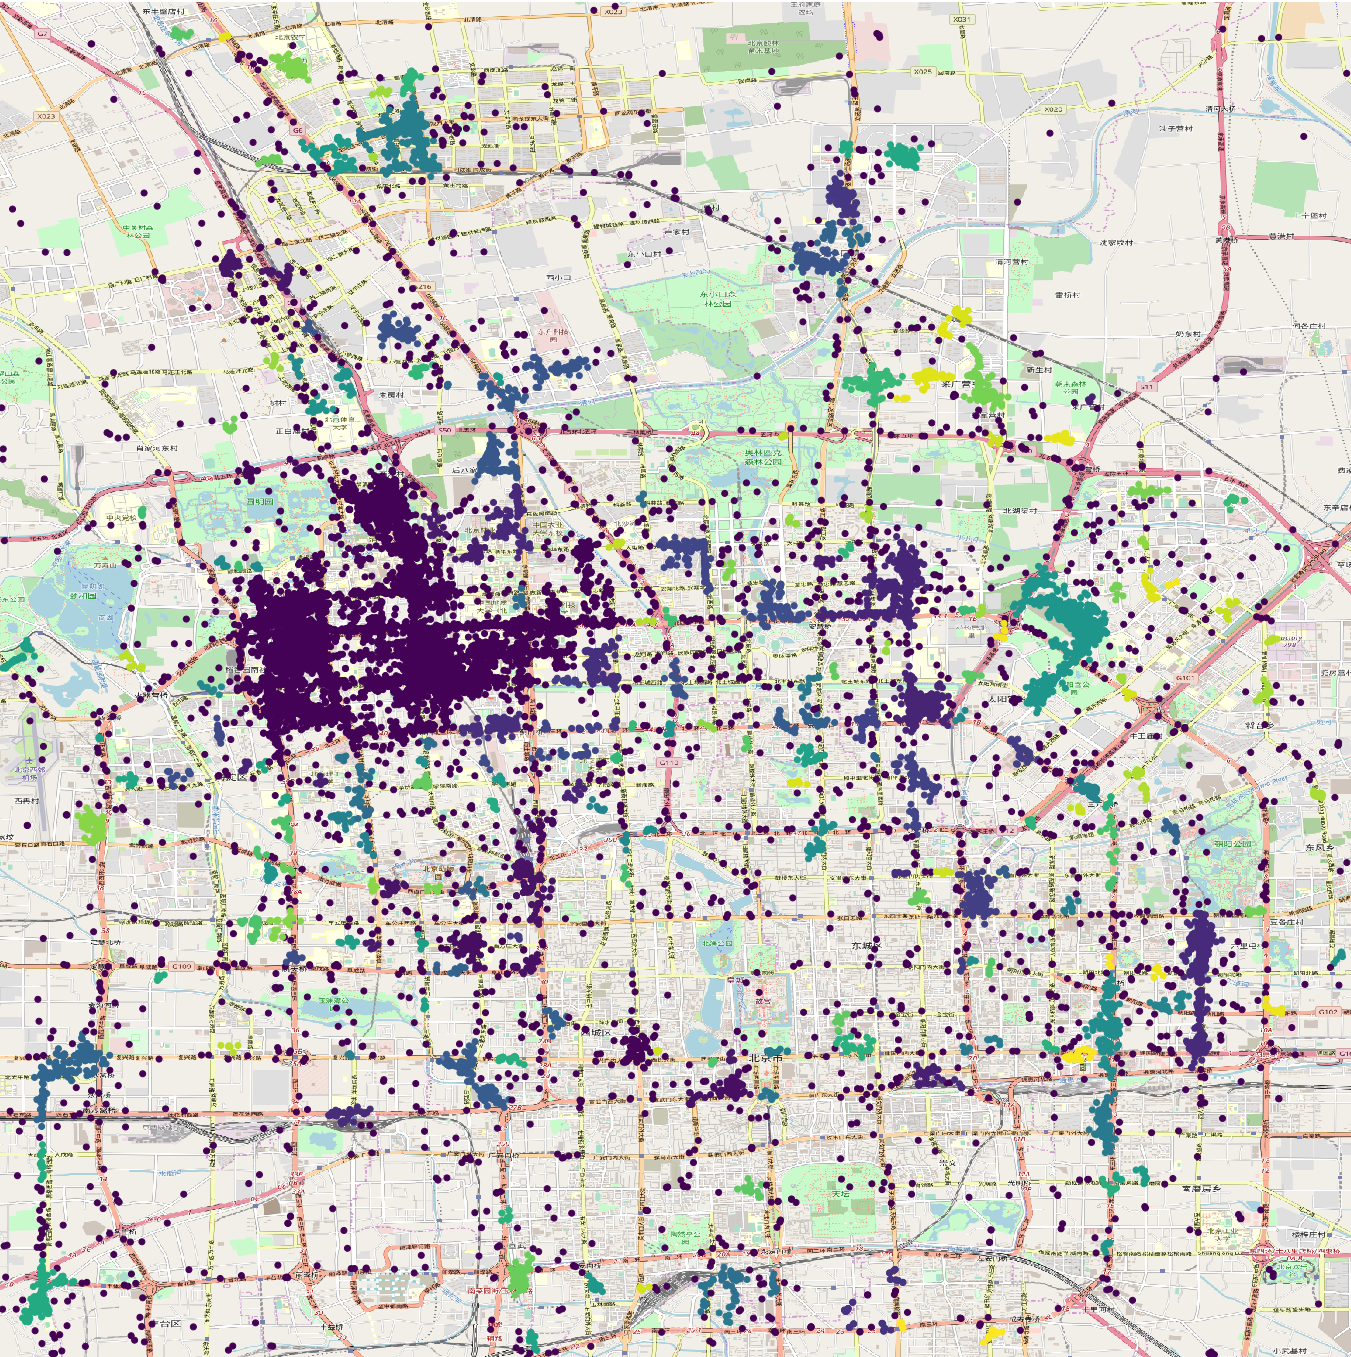
\includegraphics[height=7.5cm]{figures/cluttered_map}
\end{column}
\end{columns}
\end{frame}

\begin{frame}{Trouver les points d'intérêt à Beijing}
\begin{columns}
\begin{column}{0.5\textwidth}
\begin{description}
	\item [2.] Enlever les points ne faisant pas partie des 10 plus grands \textit{clusters}
\end{description}
\end{column}
\begin{column}{0.5\textwidth}  %%<--- here
     \centering
	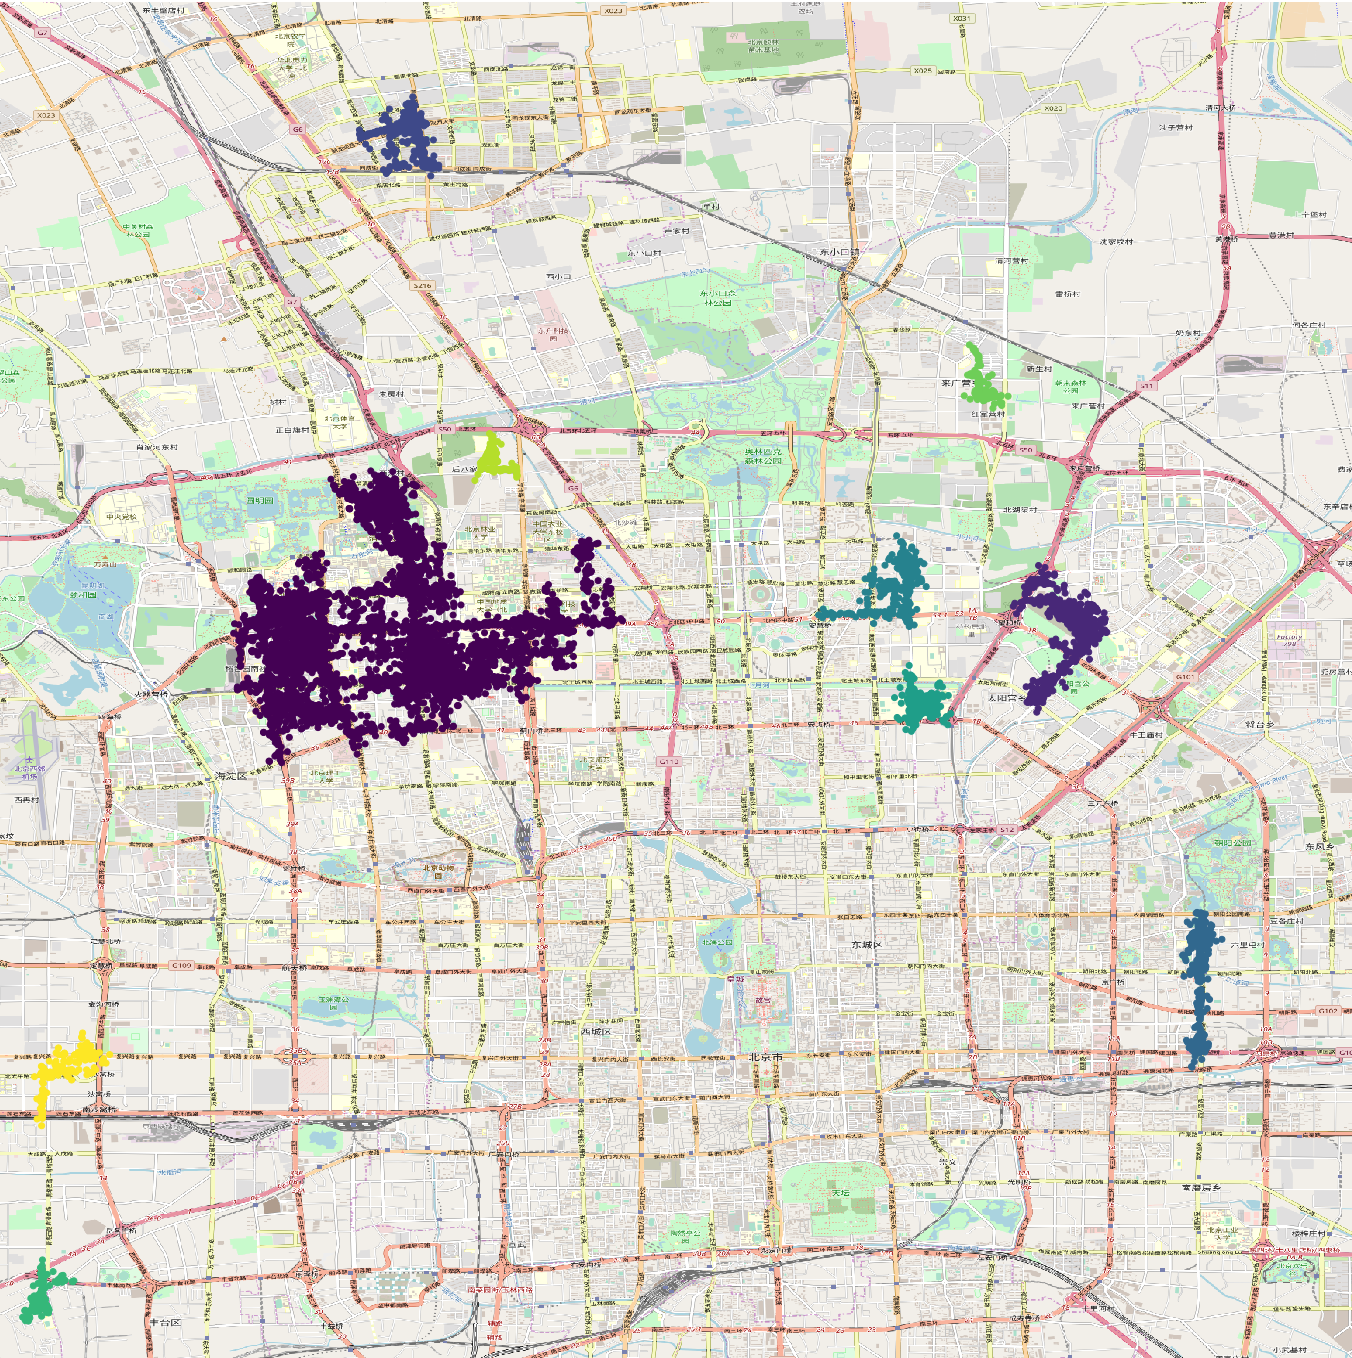
\includegraphics[height=7.5cm]{figures/reduced_map}
\end{column}
\end{columns}
\end{frame}

\begin{frame}{Trouver les points d'intérêt à Beijing}
\begin{columns}
\begin{column}{0.5\textwidth}
\begin{description}
	\item [3.] Trouver le centroïde de chaque \textit{cluster}
\end{description}
\end{column}
\begin{column}{0.5\textwidth}  %%<--- here
     \centering
	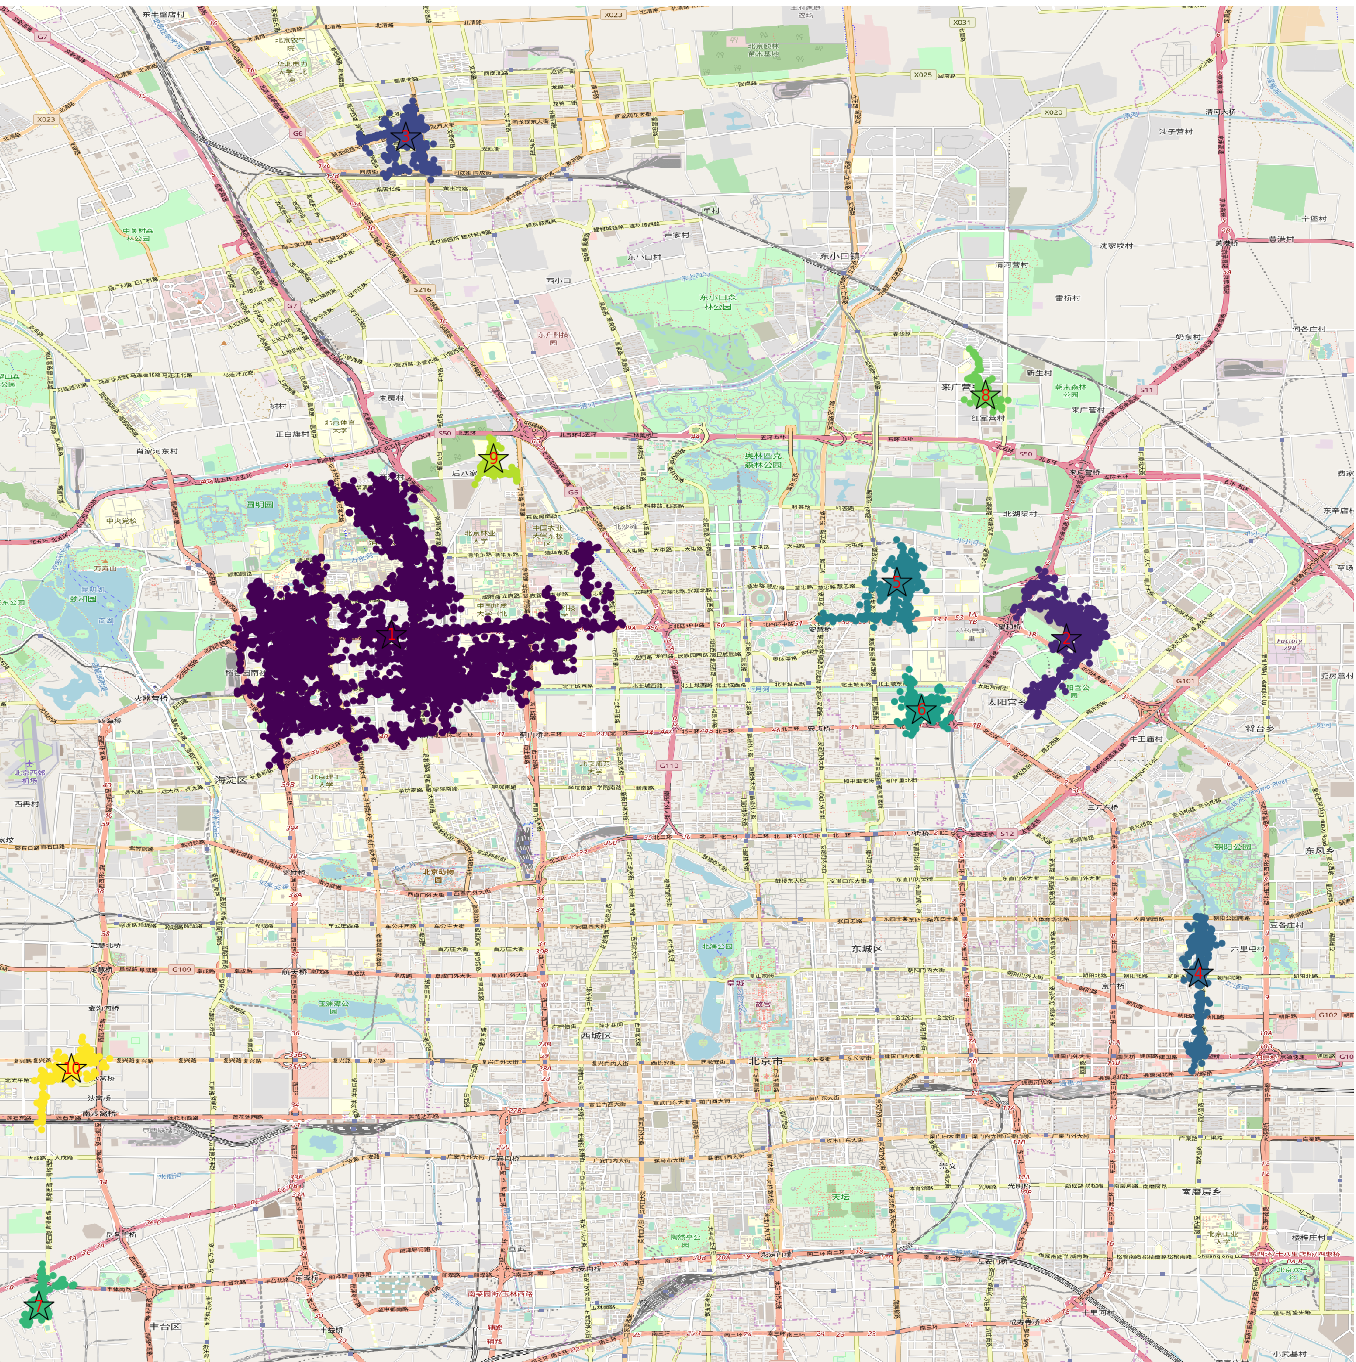
\includegraphics[height=7.5cm]{figures/annotated_map}
\end{column}
\end{columns}
\end{frame}

\begin{frame}{Trouver les points d'intérêt à Beijing}
\begin{center}
\begin{description}
	\item [4.] Utiliser le géocodage inversé (reverse geocoding) pour trouver les points d'intérêt proche des centroïdes
\end{description}
{\small \verbatiminput{scripts/reverse_geocoding.txt}}
\end{center}
\end{frame}

\begin{frame}{Finding hotspots in Beijing}

{\Large Améliorations possibles}
\vspace{.5cm}
\begin{itemize}
	\item Faire des \textit{clusters} plus petits pour améliorer les résultats du géocodage inversé
	\item Trouver une manière de trouver le point d'intérêt associé au \textit{clusters} et pas seulement le nom de la rue
	\item Regarder si les \textit{clusters} changent en fonction de l'heure de la journée, de la journée dans la semaine, ...
	\item Trouver les \textit{clusters} associés à un seul usager pour trouver ses endroits souvent fréquentés (ex. sa maison, son travail, etc.)
\end{itemize}
\end{frame}

%%%%%%%%%%%%%%%%%%%%%%%%%%%%%%%%%%%%%%%%%%%%%%%%%%%%%%%%%%%%%%%%%%%%%%%%%%%%%%%%%%%%%%%%
% Destination Prediction
%%%%%%%%%%%%%%%%%%%%%%%%%%%%%%%%%%%%%%%%%%%%%%%%%%%%%%%%%%%%%%%%%%%%%%%%%%%%%%%%%%%%%%%%

\section{Prédire la destination d'un conducteur}

\begin{frame}{Prédire la destination d'un conducteur}

\begin{center}
{\LARGE Prédire la destination d'un conducteur}
\end{center}

On peut essayer de prédire la destination d'un conducteur en fonction du début de son trajet.
\vspace{.5cm}

\begin{itemize}
	\item Plusieurs personnes ont essayé de s'attaquer à ce problème avec divers degré de succès. \cite{de2015artificial, krumm2006predestination}.
	\item On va utiliser un réseau de neurones LSTM pour faire la prédiction.
\end{itemize}
\end{frame}

\begin{frame}{Prédire la destination d'un conducteur}

{\Large Introduction rapide aux réseaux de neurones}

\begin{itemize}
	\item Modèle d'apprentissage automatique nous permettant d'apprendre des fonctions non-linéaires
	\item Peut être utilisé pour la régression (cible $\in \mathbb{R}$) et la classification (cible$\in \{1, \dots, N\}$).
\end{itemize}
\centering
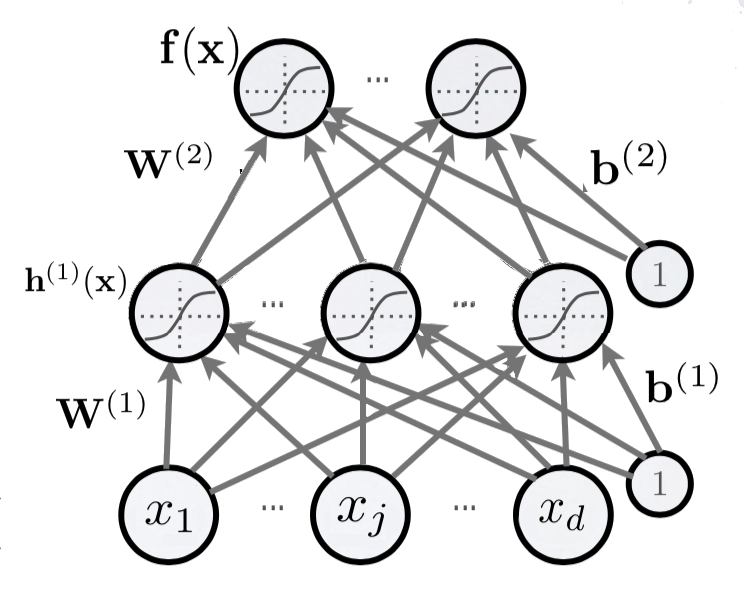
\includegraphics[height=4cm]{figures/nn}

Pour plus de détails : \url{http://cs231n.github.io/neural-networks-1/#nn}

\end{frame}

\begin{frame}{Prédire la destination d'un conducteur}

{\Large Introduction rapide aux réseaux de neurones}

\begin{itemize}
	\item Les \textbf{réseaux de neurones récurrents (RNN)} peuvent prendre en entrée des séquences de longueur variable.
	\item Idéal lorsque les données présentent des dépendances temporelles
	\item \textbf{Limitations} : Peuvent avoir de la difficulté à apprendre des dépendances à long-terme
\end{itemize}
\centering
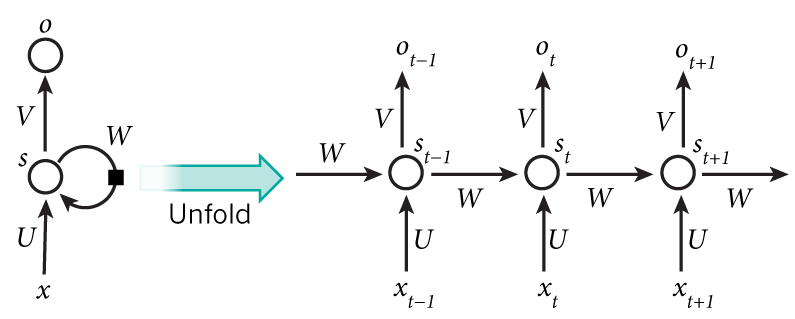
\includegraphics[width=0.6\textwidth]{figures/rnn}

Pour plus de détails : \url{http://karpathy.github.io/2015/05/21/rnn-effectiveness/}

\end{frame}

\begin{frame}{Prédire la destination d'un conducteur}

{\Large Introduction rapide aux réseaux de neurones}

\begin{itemize}
	\item Les réseaux \textbf{Long Short-Term Memory}(LSTM) peuvent apprendre ces dépendances à long-terme plus facilement.
\end{itemize}
\centering
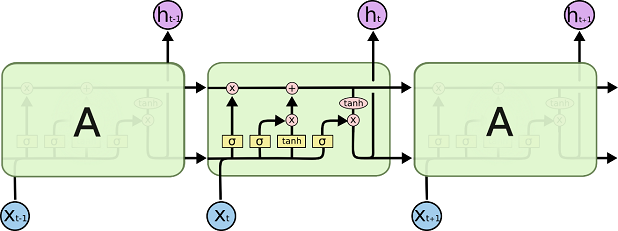
\includegraphics[width=0.6\textwidth]{figures/lstm}

Pour plus de détails : \url{https://colah.github.io/posts/2015-08-Understanding-LSTMs/}

\end{frame}

\begin{frame}{Prédire la destination d'un conducteur}

{\Large Notre approche}

\begin{itemize}
	\item On fournit en entrée une séquence de longueur de variable de tuples (lat, long) au modèle.
	\item On fournit la moitié du trajet pour faire la prédiction.
	\item On essaie de prédire la position géographique \textit{(lat, long)}de la destination.
	\item C'est un problème de régression.
	\item On optimise le modèle en essayant de minimiser la distance entre la destination prédite ainsi que la vraie destination.
\end{itemize}
\end{frame}

\begin{frame}{Predicting a driver's destination}
\centering
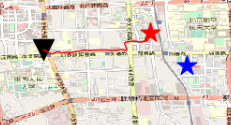
\includegraphics[width=0.6\textwidth]{figures/ex1_reg}
\end{frame}

\begin{frame}{Prédire la destination d'un conducteur}
\centering
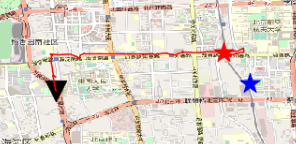
\includegraphics[width=0.6\textwidth]{figures/ex2_reg}
\end{frame}

\begin{frame}{Prédire la destination d'un conducteur}
\centering
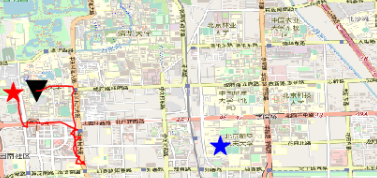
\includegraphics[width=0.6\textwidth]{figures/ex3_reg}
\end{frame}

\begin{frame}{Prédire la destination d'un conducteur}
\centering
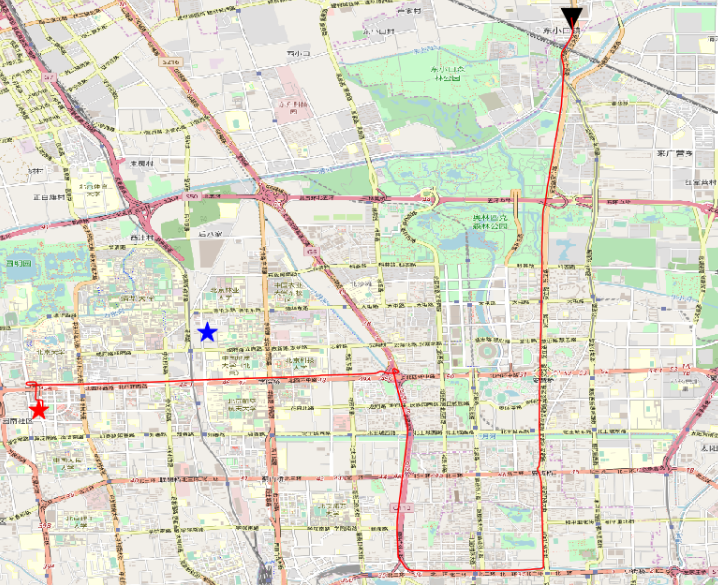
\includegraphics[width=0.6\textwidth]{figures/ex4_reg}
\end{frame}

\begin{frame}{Prédire la destination d'un conducteur}

{\Large Problèmes}

\begin{itemize}
	\item Le modèle prédit toujours des points dans le plus grand \textit{cluster} des destinations vu précédemment.
	\item C'est le "Safe bet" pour réduire la distance entre la destination prédite et la vraie destination.
	\item Le modèle n'a aucune information à propos du réseau routier à toutes les trajets se produisent.
\end{itemize}
\end{frame}

\begin{frame}{Prédire la destination d'un conducteur}

{\Large Notre deuxième essai}

\begin{itemize}
	\item On fournit en entrée une séquence de longueur de variable de tuples (lat, long) au modèle.
	\item On fournit la moitié du trajet pour faire la prédiction.
	\item On essaie de prédire le noeud du réseau routier le plus rapproché de la destination.
	\item C'est maintenant un problème de classification.
\end{itemize}
\end{frame}

\begin{frame}{Prédire la destination d'un conducteur}
\centering
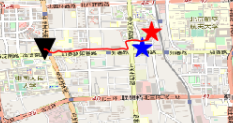
\includegraphics[width=0.6\textwidth]{figures/ex1_clf}
\end{frame}

\begin{frame}{Prédire la destination d'un conducteur}
\centering

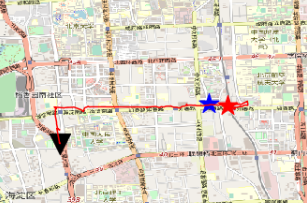
\includegraphics[width=0.6\textwidth]{figures/ex2_clf}
\end{frame}

\begin{frame}{Prédire la destination d'un conducteur}
\centering

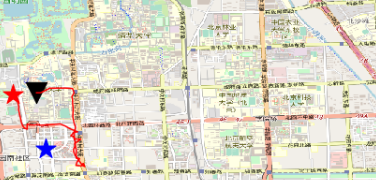
\includegraphics[width=0.6\textwidth]{figures/ex3_clf}
\end{frame}

\begin{frame}{Prédire la destination d'un conducteur}
\centering

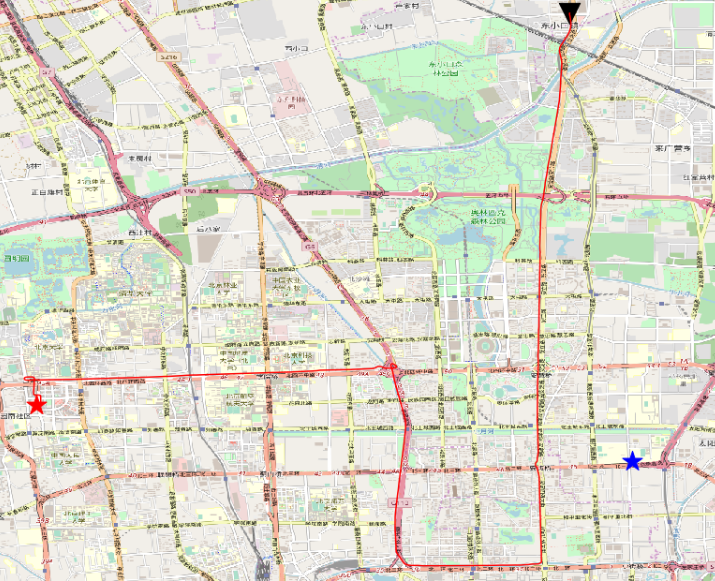
\includegraphics[width=0.6\textwidth]{figures/ex4_clf}
\end{frame}

\begin{frame}{Prédire la destination d'un conducteur}

{\Large Améliorations possibles}

\vspace{.5cm}
\begin{itemize}
	\item Ajouter le temps de la journée ou le jour de la semaine comme \textit{feature} pour chaque point.
	\item Utiliser les noeuds du réseau routier au lieu des données GPS brutes comme entrée ("node embeddings")
	\item Caractériser comment l'erreur évolue en fonction de la fraction du trajet qu'on donne en entrée au modèle.
\end{itemize}

\end{frame}

%%%%%%%%%%%%%%%%%%%%%%%%%%%%%%%%%%%%%%%%%%%%%%%%%%%%%%%%%%%%%%%%%%%%%%%%%%%%%%%%%%%%%%%%
% Geospatial Data Science at Intact
%%%%%%%%%%%%%%%%%%%%%%%%%%%%%%%%%%%%%%%%%%%%%%%%%%%%%%%%%%%%%%%%%%%%%%%%%%%%%%%%%%%%%%%%

\section{Science des données géospatiales chez  Intact}

\begin{frame}{Science des données géospatiales chez Intact}
\begin{itemize}
	\item L'équipe UBI (\textit{Usage Based Insurance}) chez Intact essaie de mieux comprendre le comportement des usagers de la route en fonction de leurs habitudes de conduite.
	\vspace{.5cm}
	\item On utilise de grandes quantités de données géospatiales pour :
	\begin{itemize}
		\item Détecter des comportements dangereux ou hors du commun sur la route
		\item Détecter des rues ou intersections dangereuses où les accidents sont plus fréquents
		\item Aider les usagers à améliorer leur conduite via une application mobile
	\end{itemize}
	\vspace{.5cm}
	\item Nous sommes toujours à la recherche de stagiaires!
\end{itemize}

\centering
\href{https://careers.intact.ca/ca/en/}{
\includegraphics[width=.2\textwidth]{figures/intact_logo}}
\end{frame}

%%%%%%%%%%%%%%%%%%%%%%%%%%%%%%%%%%%%%%%%%%%%%%%%%%%%%%%%%%%%%%%%%%%%%%%%%%%%%%%%%%%%%%%%
% References
%%%%%%%%%%%%%%%%%%%%%%%%%%%%%%%%%%%%%%%%%%%%%%%%%%%%%%%%%%%%%%%%%%%%%%%%%%%%%%%%%%%%%%%%

\section*{References}

\begin{frame}[t,allowframebreaks]
\setbeamertemplate{bibliography item}{[\theenumiv]}


  \frametitle{Références}
  \nocite*
  \bibliographystyle{siam}
  \bibliography{references}
 \end{frame}

\end{document}